% !TEX root = ../main.tex
% =============================================================================
% CHAPTER 2 - BACKGROUND (target ~9-10 pages)
% Tense: present tense (established, timeless knowledge). Use simple past only when
% describing what a SPECIFIC prior study did. Define every acronym on first use.
% Support every claim with a citation.
% =============================================================================
\chapter{Background}\label{ch:background}

This chapter introduces the technical and clinical concepts required to understand the methods and experiments in this thesis, including resting-state EEG, the clinical conditions considered, self-supervised representation learning, EEG microstates, and positional encoding.


\section{Electroencephalography}\label{sec:bg_eeg}

\subsection{EEG Basics}

\begin{figure}[htbp]
\centering
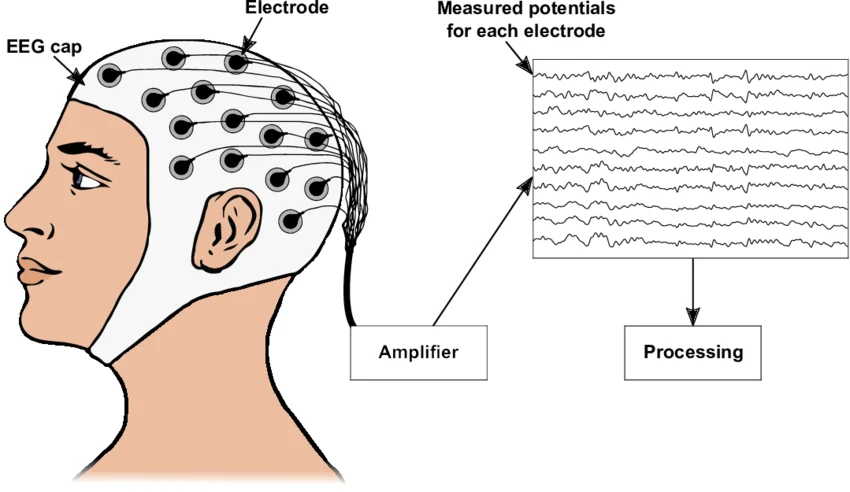
\includegraphics[width=0.68\textwidth]{figures/fig_eeg_recording.png}
\caption[The EEG recording chain]{EEG recording chain from scalp electrodes to digitised time series. Reproduced from \textcite{nagelTowardsHomeuseBCI2019}.}
\label{fig:eeg_recording}
\end{figure}

Electroencephalography (EEG) is a non-invasive method for recording electrical brain activity from electrodes placed on the scalp. It provides high temporal resolution, allowing changes in brain activity to be measured at the millisecond scale. The recorded voltages mainly reflect the combined postsynaptic activity of large populations of cortical neurons. As these electrical fields travel through brain tissue, cerebrospinal fluid, skull, and scalp before reaching the electrodes, each EEG channel reflects a mixture of activity from multiple neural sources rather than a single isolated source \parencite{jacksonNeurophysiologicalBasesEEG2014}. In practice the scalp potentials are picked up by electrodes held against the head, amplified, and digitised, giving one time series per electrode for subsequent analysis, as shown in Figure~\ref{fig:eeg_recording}.


Electrodes are commonly positioned using the international 10-20 system \parencite{homan1020ElectrodeSystem1988}, which defines reproducible locations over the scalp. Electrode positions are defined relative to standard anatomical landmarks on the head, ensuring consistent placement across participants. Figure~\ref{fig:eeg_montage} shows these landmarks and the denser 10-10 extension, within which the 19 electrodes used throughout this thesis (Section~\ref{sec:m_brainlmeeg}) are located. The set of recorded electrodes and the reference scheme together define the montage. The reference is important because EEG measures voltage differences rather than absolute voltage. Changing the reference therefore changes the recorded channel values and can affect relationships between channels \parencite{bigdely-shamloPREPPipelineStandardized2015a}.


\begin{figure}[htbp]
\centering
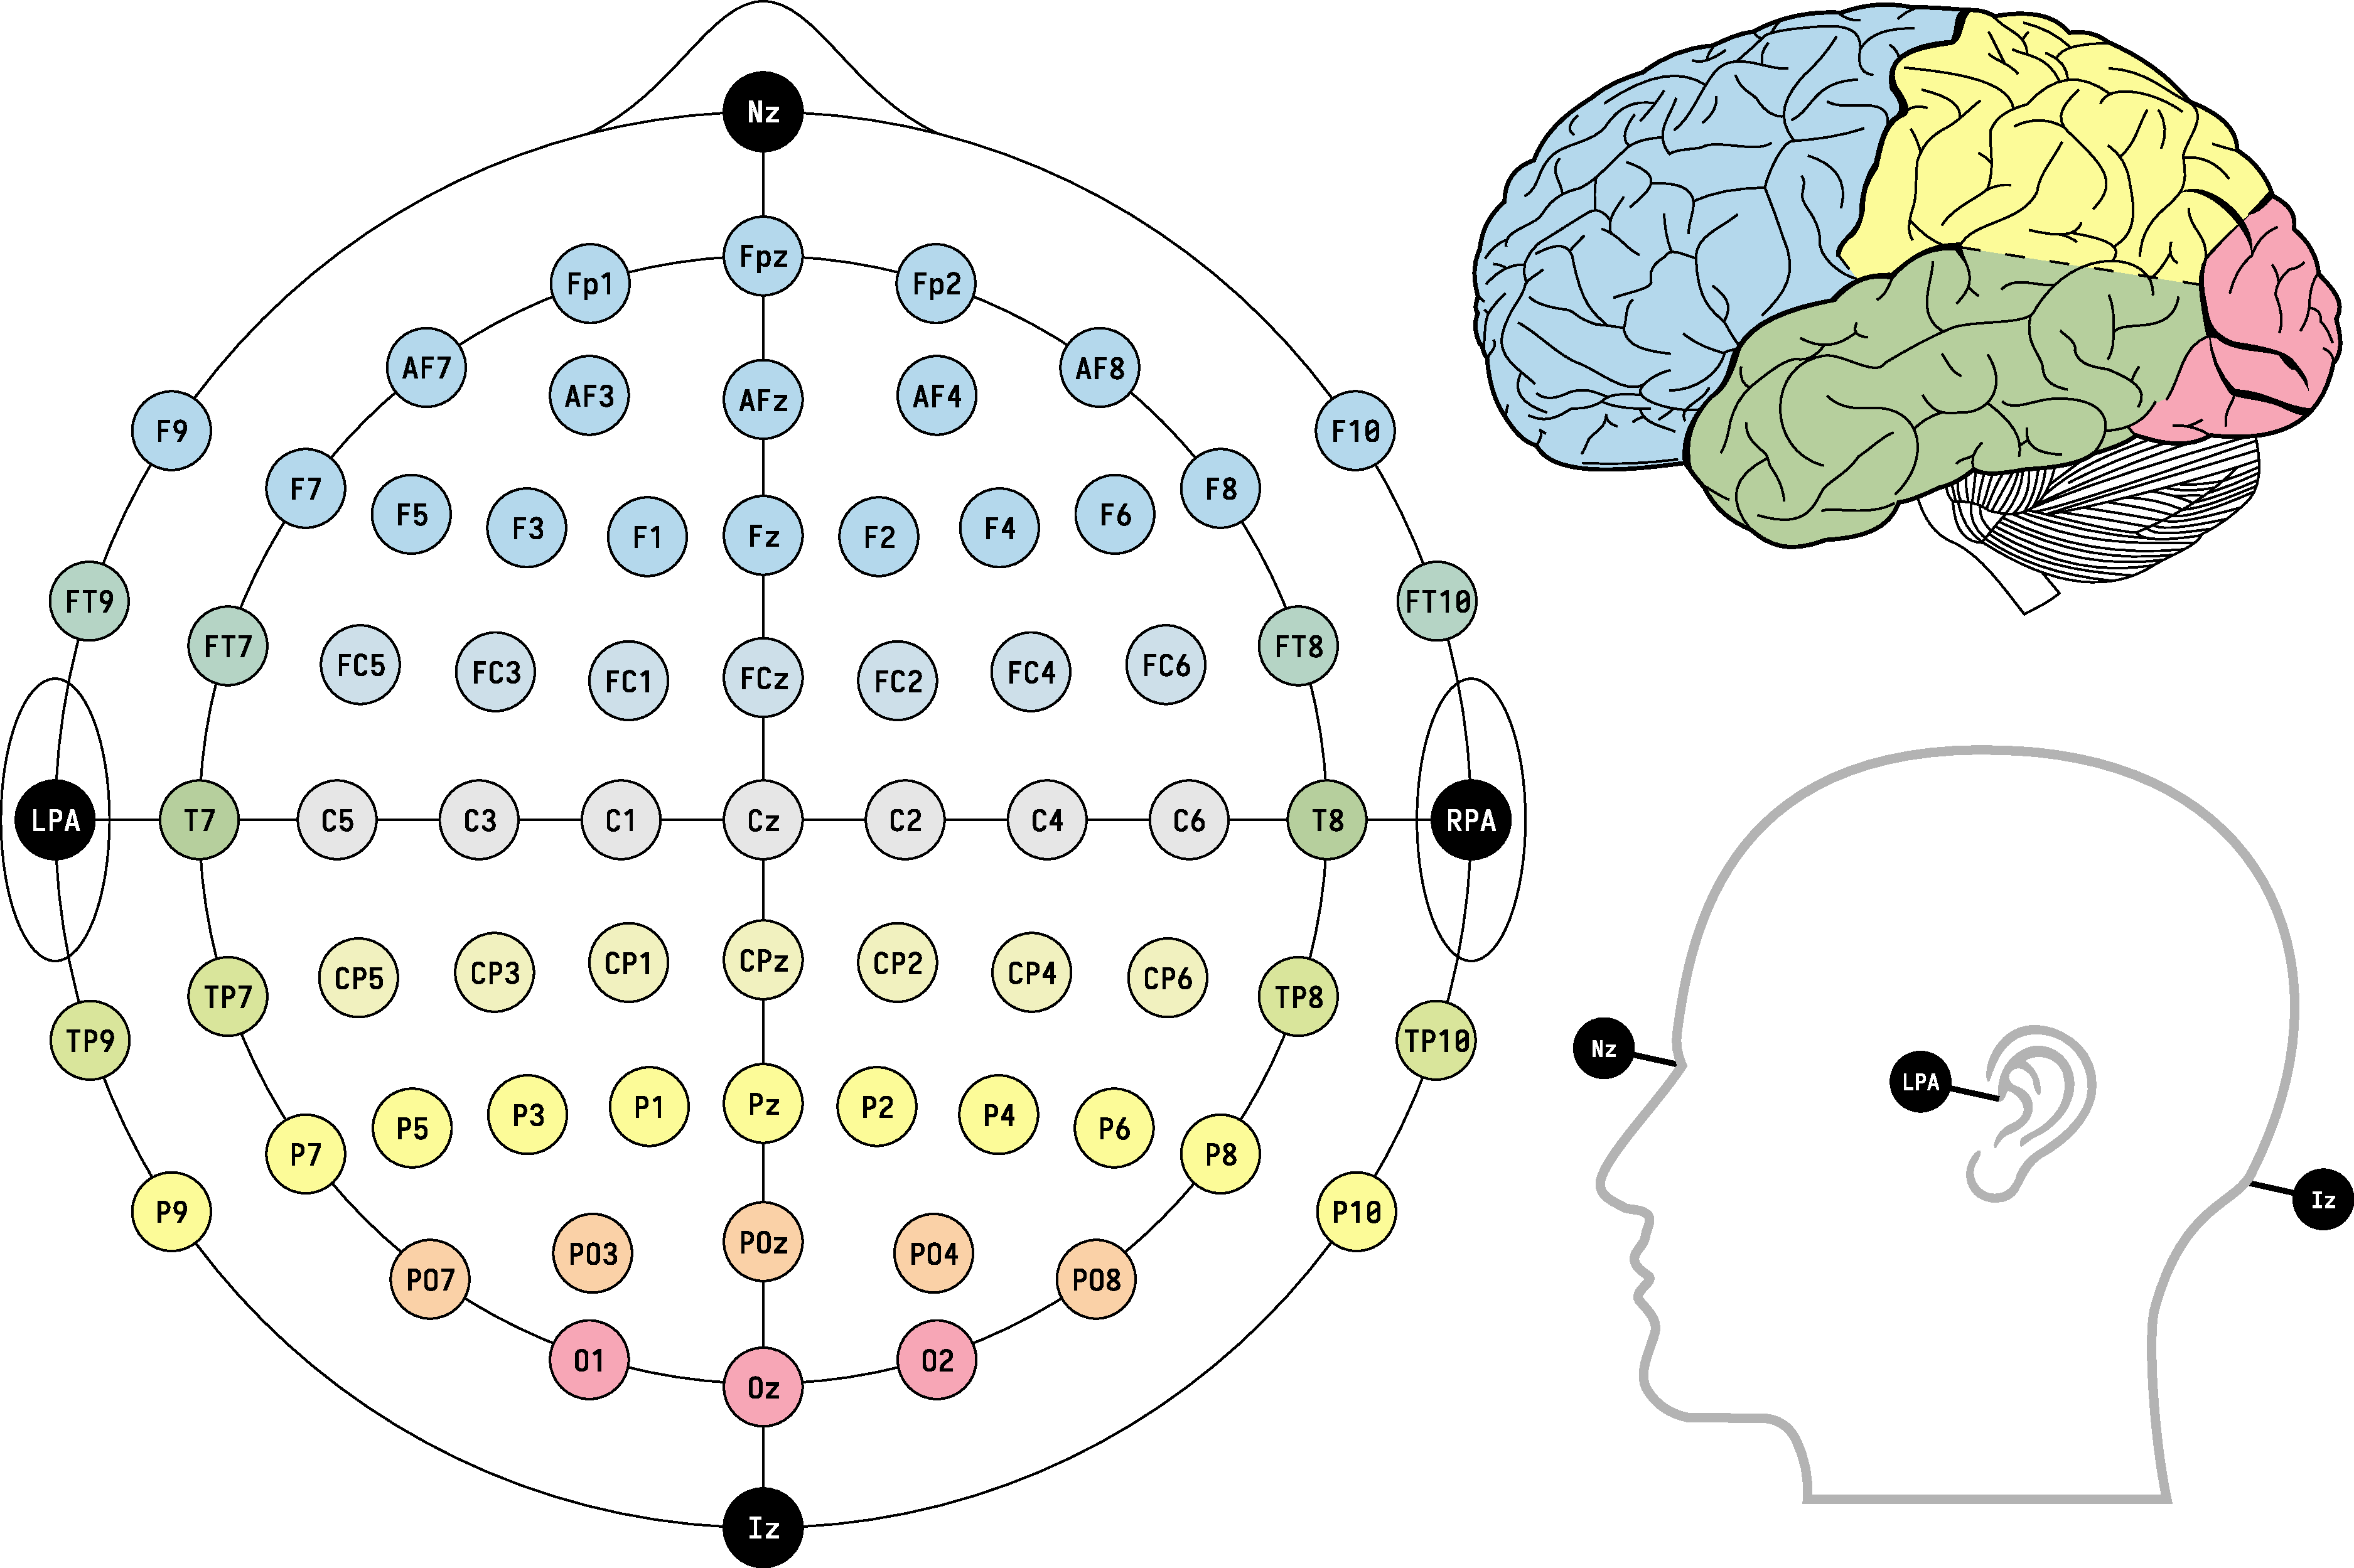
\includegraphics[width=0.90\textwidth]{figures/fig_eeg_montage.pdf}
\caption[Electrode positions of the 10-10 system]{Electrode positions of the international 10-10 system, an extension of the 10-20 system. Labels follow the modified combinatorial nomenclature. Figure by Laurens R. Krol, released into the public domain under CC0 1.0 \parencite{krolEEG1010System2020}.}
\label{fig:eeg_montage}
\end{figure}

EEG is therefore a multichannel signal with an inherent spatial structure. Channels are usually stored in a fixed numerical order, but this order does not describe the physical distances or directions between electrodes on the scalp. Channel identity and electrode position are related but distinct forms of information, a distinction that becomes relevant when EEG is represented as a sequence for computational models \parencite{wangCBraModCrissCrossBrain2025a,el2026reve}.

\subsection{Resting-State EEG and Frequency Bands}

Resting-state EEG is recorded while no explicit task is being performed, usually with the participant relaxed and the eyes open or closed. The two conditions are not equivalent because eye closure commonly increases posterior alpha activity and changes the distribution of resting-state rhythms \parencite{barryEEGDifferencesEyesClosed2007}. Resting-state EEG is useful in clinical research because it requires little task understanding or behavioural response.

EEG is often described through approximate frequency bands: delta at about 1-4~Hz, theta at 4-8~Hz, alpha at 8-13~Hz, beta at 13-30~Hz, and gamma above about 30~Hz. These ranges are conventions rather than fixed physiological divisions, but they provide an interpretable summary of how signal power is distributed across frequencies \parencite{teplanFundamentalsEegMeasurement2002}.

Frequency information is clinically useful because some neurological and psychiatric conditions are associated with changes in the balance between slower and faster rhythms. Alzheimer's disease (AD), for example, is commonly associated with relatively more slow activity and reduced alpha activity than healthy ageing \parencite{jeongEEGDynamicsAlzheimers2004,jelicQuantitativeElectroencephalographyPower1996}. Frequency-band summaries are interpretable, but they average activity over time and do not fully describe transient changes or relationships between electrodes.

\subsection{EEG Artefacts and Preprocessing}

Scalp EEG contains neural activity together with unwanted signals from the eyes, muscles, heart, electrodes, movement, and the electrical environment. Eye blinks can produce large slow deflections, muscle activity can add broadband high-frequency energy, and power-line interference can introduce narrow-band noise. These artefacts can be larger than the neural activity of interest \parencite{delormeEEGLABOpenSourceToolbox2004,bigdely-shamloPREPPipelineStandardized2015a}.

Preprocessing aims to reduce these effects and make recordings more comparable. Typical steps include filtering, re-referencing, detecting bad channels, and removing strongly contaminated components. Independent component analysis \parencite[ICA;][]{hyvarinenIndependentComponentAnalysis2000}, for example, separates the observed signals into components with different statistical patterns, allowing components associated with eye, cardiac, or muscle activity to be identified and removed \parencite{Li2022}.

Preprocessing is not a neutral cleaning step. Filtering changes the frequency content of the signal, re-referencing changes spatial relationships between channels, and artefact removal can also remove genuine neural activity. Differences in preprocessing and recording hardware can therefore influence the statistical properties of EEG data and complicate comparisons across datasets \parencite{bigdely-shamloPREPPipelineStandardized2015a,royDeepLearningBasedElectroencephalography2019}.

\section{Clinical Conditions}\label{sec:bg_conditions}

The clinical conditions considered in this thesis are Alzheimer's disease (AD), frontotemporal dementia (FTD), first-episode psychosis (FEP), schizophrenia (SCZ), and major depressive disorder (MDD). They differ substantially in their symptoms, disease course, and underlying pathology. Diagnosis is primarily based on clinical assessment, supported where appropriate by cognitive testing, imaging, laboratory investigations, or other biomarkers. Resting-state EEG is not a stand-alone diagnostic test for these conditions yet, but it provides a non-invasive measure of brain function that can reveal group level differences in neural activity \parencite{royDeepLearningBasedElectroencephalography2019,vanderVinneFrontalAlphaAsymmetry2017}.

\subsection{Alzheimer's Disease and Frontotemporal Dementia}\label{sec:bg_adftd}

AD and FTD are neurodegenerative disorders that progressively affect cognition and everyday functioning. AD most commonly begins with impairment of memory and gradually affects other cognitive abilities. FTD primarily affects frontal and temporal brain systems and often presents with early changes in behaviour, personality, executive function, or language. Clinical diagnosis is based on the pattern and progression of symptoms together with cognitive and neurological assessment, often supported by additional investigations \parencite{miltiadousDatasetScalpEEG2023a}.

Resting-state EEG in AD commonly shows spectral slowing, including increased relative delta and theta activity, reduced alpha activity, and a lower dominant frequency \parencite{jeongEEGDynamicsAlzheimers2004,jelicQuantitativeElectroencephalographyPower1996}. EEG findings in FTD are less uniform, although changes in functional connectivity and network organisation have been reported \parencite{dehaanFunctionalNeuralNetwork2009,yuDifferentFunctionalConnectivity2016}.

\subsection{First-Episode Psychosis and Schizophrenia}\label{sec:bg_fep}

Psychosis can involve hallucinations, delusions, and disturbances in thought or behaviour. FEP refers to the first clinical presentation of psychotic symptoms. Schizophrenia is a longer-term psychiatric disorder in which psychotic symptoms can occur together with negative symptoms, such as reduced motivation or emotional expression, and cognitive difficulties involving functions such as attention and memory. Diagnosis is based on the nature, duration, and functional impact of these symptoms rather than on an EEG measurement \parencite{uhlhaasAbnormalNeuralOscillations2010}.

EEG studies of schizophrenia report alterations in neural oscillations and in the synchronisation of activity across brain regions, although the direction and magnitude of these findings vary across cohorts and recording conditions \parencite{uhlhaasAbnormalNeuralOscillations2010}. Differences have also been reported in the temporal variability of resting-state spectral activity \parencite{raczReducedTemporalVariability2025}.

\subsection{Major Depressive Disorder}\label{sec:bg_mdd}

MDD is a psychiatric disorder characterised by persistent depressed mood, reduced interest or pleasure, or both, together with additional cognitive and physical symptoms that interfere with daily functioning. These can include changes in sleep, energy, concentration, appetite, and psychomotor activity. Diagnosis is based on the pattern, duration, and severity of symptoms and their effect on functioning \parencite{vanderVinneFrontalAlphaAsymmetry2017}.

Resting-state EEG research in MDD has examined spectral power, functional connectivity, and frontal alpha asymmetry. Frontal alpha asymmetry compares alpha activity over left and right frontal regions, but evidence for a reliable diagnostic difference between MDD and healthy controls is weak and inconsistent across studies and analysis choices \parencite{vanderVinneFrontalAlphaAsymmetry2017,kolodziejNoRelationshipFrontalAlpha2021}.

\section{Supervised Learning for EEG}\label{sec:bg_supervised}

Supervised learning uses examples for which the target label is known. In clinical EEG classification, a model receives EEG data together with a diagnostic group label and learns a mapping from the signal to that label. Classical approaches first convert EEG into hand-designed features, whereas deep models learn features directly from the signal \parencite{craikDeepLearningElectroencephalogram2019,royDeepLearningBasedElectroencephalography2019}.

\subsection{Handcrafted EEG Features and Classical Models}\label{sec:bg_classical}

A traditional EEG pipeline summarises each recording window with a feature vector. The selected features describe properties expected to be informative, such as frequency content, waveform shape, temporal variability, or relationships between electrodes. This reduces a high-dimensional time series to quantities that are easier to interpret and can work well when the number of participants is limited.

\paragraph{Spectral features.} Band power measures how much signal power lies within a selected frequency range. It is especially useful when a clinical effect changes the balance of slow and fast activity, as in AD \parencite{jeongEEGDynamicsAlzheimers2004}. Its main limitation is that averaging power over a window reduces temporal detail.

\paragraph{Time-frequency and time-domain features.} Time-domain features describe waveform properties such as variance or Hjorth activity, mobility, and complexity. Time-frequency methods describe how frequency content changes over time. Relationships between electrodes can additionally be represented through covariance, correlation, or coherence \parencite{hjorthEEGAnalysisBased1970,dehaanFunctionalNeuralNetwork2009}. These families provide complementary views of the signal.

\paragraph{Classical classifiers.} Feature vectors can be used with classifiers such as linear discriminant analysis (LDA), support vector machines (SVMs), logistic regression, or gradient-boosted trees such as XGBoost \parencite{chenXGBoostScalableTree2016}. These models remain important baselines because they are relatively data efficient. Their main limitation is that the feature set determines what information is available to the classifier.

\subsection{Deep Learning for EEG}\label{sec:bg_deep}

Deep neural networks learn feature extraction and classification jointly. Convolutional neural networks (CNNs) can learn local temporal patterns and combine information across electrodes, while transformer-based models use self-attention to model relationships between input segments over longer ranges \parencite{craikDeepLearningElectroencephalogram2019,songEEGConformerConvolutional2023a}. In EEG, the input can be divided into short channel-time segments so that the model learns from both temporal and spatial context.

Supervised deep models learn their internal representation from labelled examples. In clinical EEG, labels can be expensive to obtain and the number of independent participants is often much smaller than the number of signal segments. Self-supervised learning provides an alternative way to learn representations from unlabelled recordings before they are used for a downstream task.

\section{Self-Supervised Representation Learning}\label{sec:bg_ssl}

Self-supervised learning (SSL) creates a training target from the data itself rather than requiring a clinical label. An encoder is first trained on unlabelled EEG to solve a pretraining task. The encoder converts the input into numerical features, forming a learned representation that can later be used for labelled downstream tasks \parencite{banvilleUncoveringStructureClinical2020,kostasBENDRUsingTransformers2021}.

\subsection{Self-Supervised Learning Objectives}

A self-supervised objective determines what information the encoder is encouraged to preserve. Contrastive methods train related signal segments or transformed views to have similar representations while separating unrelated examples. Reconstruction-based methods hide or corrupt part of the input and train the model to predict the missing information from what remains \parencite{banvilleUncoveringStructureClinical2020,baevskiData2vecGeneralFramework2022}.

For EEG, the objective must be chosen carefully because nearby time samples and neighbouring channels are strongly related. A task that is too easy may be solved by local interpolation, while a task dominated by noise may encourage the model to reconstruct artefacts rather than useful brain activity. The pretraining objective therefore shapes what information becomes available in the learned representation.

\subsection{Masked Autoencoders}

A masked autoencoder \parencite[MAE;][]{heMaskedAutoencodersAre2022} divides an input into patches, masks a subset of them, and reconstructs the missing content from the remaining visible patches. The encoder processes only the visible patches, while the decoder receives their latent representations together with mask tokens and positional information to reconstruct the masked patches. The reconstruction objective encourages the encoder to capture dependencies between visible and masked parts of the input that are useful for inferring missing information.

The masked reconstruction principle can also be applied to sequential and multivariate signals, including recordings of brain activity. The representations learned through this process are influenced by how the signal is partitioned into patches, which patches are masked, and how positional or spatial information is encoded. These choices are particularly relevant for multichannel EEG, where information varies across both time and electrode location. Chapter~\ref{ch:related} reviews how existing EEG representation learning models address these design choices.


\section{EEG Microstates}\label{sec:bg_microstates}

Frequency bands describe how signal power is distributed across frequencies, but they do not directly describe the shape of the electrical field over the scalp at a particular moment. EEG microstates provide a complementary description. A microstate is a short period during which the spatial pattern of scalp voltages remains approximately stable before changing to another pattern \parencite{391164,michelEEGMicrostatesTool2018a}.

Microstate analysis reduces continuous multichannel EEG to a sequence of recurring scalp maps. Representative topographies are identified and then matched back to the recording, allowing the sequence to be described by properties such as duration, occurrence, coverage, and transitions \parencite{391164,Férat2022}. Common labels such as A, B, C, and D are names for recurring topographic patterns rather than fixed brain regions or disease classes. Their exact form depends on preprocessing and template estimation \parencite{Férat2022,khannaReliabilityRestingStateMicrostate2014a}. Figure~\ref{fig:microstate_maps} shows the four maps estimated for this thesis, which are used as prediction targets by one of the model variants introduced in Section~\ref{sec:m_microstate}.

% Drawn from metadata/microstates/canonical_maps.npz, the same file
% brainlm_microstate.py loads at construction time. Generated by
% code/analysis/dataset/generate_model_figures.py; do not resize here.
\begin{figure}[htbp]
\centering
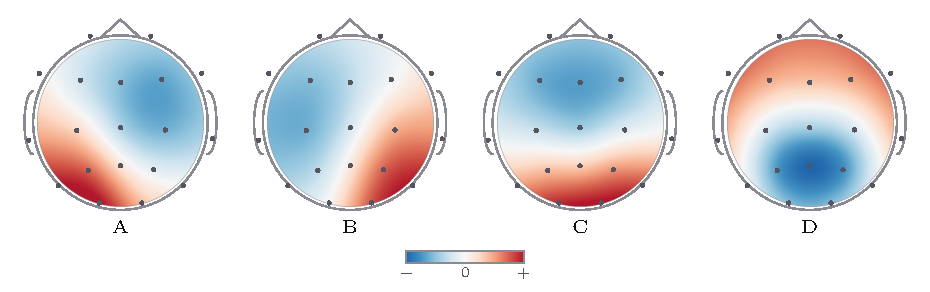
\includegraphics[width=\textwidth]{figures/fig_microstate_maps.pdf}
\caption[The four canonical microstate maps]{The four canonical microstate maps (A-D) used in this thesis, estimated from the LEMON training partition (Section~\ref{sec:m_microstate}). Each map is defined by one value at each of the 19 electrodes (dots); the continuous colour field between electrodes is obtained by spatial interpolation for visualisation. Colour indicates relative scalp potential from negative (blue) to positive (red).}
\label{fig:microstate_maps}
\end{figure}


\section{Positional Encoding in Transformer Models}\label{sec:bg_posenc}

Self-attention \parencite{vaswaniAttentionAllYou2017} does not inherently encode the order or position of input tokens, so Transformer models require an additional mechanism for representing positional information \parencite{dufterPositionInformationTransformers2021}. For EEG, positional information can have both temporal and spatial components: temporal position describes when a patch occurs within the recording, while spatial position describes the location of its corresponding electrode on the scalp.

A learned channel embedding can distinguish electrodes within a fixed montage, but it represents channel identity as a learned label rather than explicitly encoding the physical relationships between electrode locations. This distinction becomes relevant when electrode configurations differ across datasets, because learned channel embeddings are tied to the channel identities encountered during training and do not explicitly represent relative electrode geometry. Coordinate-based encodings instead represent electrodes using their spatial coordinates rather than their position in an arbitrary channel ordering. Rotary positional embedding \parencite[RoPE;][]{suRoFormerEnhancedTransformer2024} incorporates positional information into self-attention by applying position-dependent rotations to query and key representations, such that their interaction reflects relative positional relationships. RoPE has also been extended to multidimensional coordinates \parencite{heoRotaryPositionEmbedding2025}, allowing spatial relationships to be represented in more than one dimension.
